\documentclass[convert={density=1200}]{standalone}
\usepackage{tikz}
\usetikzlibrary{shapes.geometric, arrows}

\tikzstyle{server} = [rectangle, rounded corners, text centered, draw=black, fill=green!30, inner sep=5pt]
\tikzstyle{node} = [rectangle, rounded corners, text centered, draw=black, fill=blue!30, inner sep=5pt]
\tikzstyle{arrow1} = [thick, ->, >=stealth]
\tikzstyle{arrow2} = [blue, dashed, ->, >=stealth]

\begin{document}

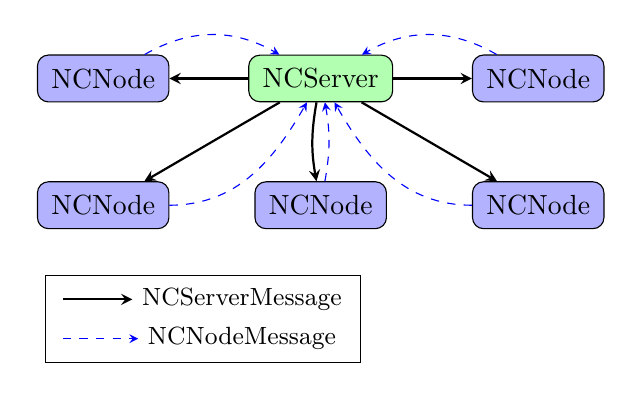
\begin{tikzpicture}

    \matrix [column sep = 10mm, row sep = 10mm] {
        \node (ncnode1) [node] {NCNode}; &
        \node (ncserver) [server] {NCServer}; &
        \node (ncnode2) [node] {NCNode}; \\
        \node (ncnode3) [node] {NCNode}; &
        \node (ncnode4) [node] {NCNode}; &
        \node (ncnode5) [node] {NCNode}; \\
    };

    \draw [arrow1] (ncserver) -- (ncnode1);
    \draw [arrow1] (ncserver) -- (ncnode2);
    \draw [arrow1] (ncserver) -- (ncnode3);
    \draw [arrow1] (ncserver) to [out=260, in=100] (ncnode4);
    \draw [arrow1] (ncserver) -- (ncnode5);

    \draw [arrow2] (ncnode1) to [out=30, in=150] (ncserver);
    \draw [arrow2] (ncnode2) to [out=150, in=30] (ncserver);
    \draw [arrow2] (ncnode3) to [out=0, in=240] (ncserver);
    \draw [arrow2] (ncnode5) to [out=180, in=300] (ncserver);
    \draw [arrow2] (ncnode4) to [out=80, in=280] (ncserver);

    \draw [white] (-1, -2.9) rectangle (1, -2.8);

    \draw (-3.5, -2.8) rectangle (0.5, -1.7);

    \node (label1a) at (-3.4, -2) {};
    \node [font=\small] (label1b) at (-1, -2) {NCServerMessage};

    \draw [arrow1] (label1a) -- (label1b);

    \node (label2a) at (-3.4, -2.5) {};
    \node [font=\small] (label2b) at (-1, -2.5) {NCNodeMessage};

    \draw [arrow2] (label2a) -- (label2b);

\end{tikzpicture}

\end{document}
